\documentclass[1p]{elsarticle_modified}
%\bibliographystyle{elsarticle-num}

%\usepackage[colorlinks]{hyperref}
%\usepackage{abbrmath_seonhwa} %\Abb, \Ascr, \Acal ,\Abf, \Afrak
\usepackage{amsfonts}
\usepackage{amssymb}
\usepackage{amsmath}
\usepackage{amsthm}
\usepackage{scalefnt}
\usepackage{amsbsy}
\usepackage{kotex}
\usepackage{caption}
\usepackage{subfig}
\usepackage{color}
\usepackage{graphicx}
\usepackage{xcolor} %% white, black, red, green, blue, cyan, magenta, yellow
\usepackage{float}
\usepackage{setspace}
\usepackage{hyperref}

\usepackage{tikz}
\usetikzlibrary{arrows}

\usepackage{multirow}
\usepackage{array} % fixed length table
\usepackage{hhline}

%%%%%%%%%%%%%%%%%%%%%
\makeatletter
\renewcommand*\env@matrix[1][\arraystretch]{%
	\edef\arraystretch{#1}%
	\hskip -\arraycolsep
	\let\@ifnextchar\new@ifnextchar
	\array{*\c@MaxMatrixCols c}}
\makeatother %https://tex.stackexchange.com/questions/14071/how-can-i-increase-the-line-spacing-in-a-matrix
%%%%%%%%%%%%%%%

\usepackage[normalem]{ulem}

\newcommand{\msout}[1]{\ifmmode\text{\sout{\ensuremath{#1}}}\else\sout{#1}\fi}
%SOURCE: \msout is \stkout macro in https://tex.stackexchange.com/questions/20609/strikeout-in-math-mode

\newcommand{\cancel}[1]{
	\ifmmode
	{\color{red}\msout{#1}}
	\else
	{\color{red}\sout{#1}}
	\fi
}

\newcommand{\add}[1]{
	{\color{blue}\uwave{#1}}
}

\newcommand{\replace}[2]{
	\ifmmode
	{\color{red}\msout{#1}}{\color{blue}\uwave{#2}}
	\else
	{\color{red}\sout{#1}}{\color{blue}\uwave{#2}}
	\fi
}

\newcommand{\Sol}{\mathcal{S}} %segment
\newcommand{\D}{D} %diagram
\newcommand{\A}{\mathcal{A}} %arc


%%%%%%%%%%%%%%%%%%%%%%%%%%%%%5 test

\def\sl{\operatorname{\textup{SL}}(2,\Cbb)}
\def\psl{\operatorname{\textup{PSL}}(2,\Cbb)}
\def\quan{\mkern 1mu \triangleright \mkern 1mu}

\theoremstyle{definition}
\newtheorem{thm}{Theorem}[section]
\newtheorem{prop}[thm]{Proposition}
\newtheorem{lem}[thm]{Lemma}
\newtheorem{ques}[thm]{Question}
\newtheorem{cor}[thm]{Corollary}
\newtheorem{defn}[thm]{Definition}
\newtheorem{exam}[thm]{Example}
\newtheorem{rmk}[thm]{Remark}
\newtheorem{alg}[thm]{Algorithm}

\newcommand{\I}{\sqrt{-1}}
\begin{document}

%\begin{frontmatter}
%
%\title{Boundary parabolic representations of knots up to 8 crossings}
%
%%% Group authors per affiliation:
%\author{Yunhi Cho} 
%\address{Department of Mathematics, University of Seoul, Seoul, Korea}
%\ead{yhcho@uos.ac.kr}
%
%
%\author{Seonhwa Kim} %\fnref{s_kim}}
%\address{Center for Geometry and Physics, Institute for Basic Science, Pohang, 37673, Korea}
%\ead{ryeona17@ibs.re.kr}
%
%\author{Hyuk Kim}
%\address{Department of Mathematical Sciences, Seoul National University, Seoul 08826, Korea}
%\ead{hyukkim@snu.ac.kr}
%
%\author{Seokbeom Yoon}
%\address{Department of Mathematical Sciences, Seoul National University, Seoul, 08826,  Korea}
%\ead{sbyoon15@snu.ac.kr}
%
%\begin{abstract}
%We find all boundary parabolic representation of knots up to 8 crossings.
%
%\end{abstract}
%\begin{keyword}
%    \MSC[2010] 57M25 
%\end{keyword}
%
%\end{frontmatter}

%\linenumbers
%\tableofcontents
%
\newcommand\colored[1]{\textcolor{white}{\rule[-0.35ex]{0.8em}{1.4ex}}\kern-0.8em\color{red} #1}%
%\newcommand\colored[1]{\textcolor{white}{ #1}\kern-2.17ex	\textcolor{white}{ #1}\kern-1.81ex	\textcolor{white}{ #1}\kern-2.15ex\color{red}#1	}

{\Large $\underline{12n_{0561}~(K12n_{0561})}$}

\setlength{\tabcolsep}{10pt}
\renewcommand{\arraystretch}{1.6}
\vspace{1cm}\begin{tabular}{m{100pt}>{\centering\arraybackslash}m{274pt}}
\multirow{5}{120pt}{
	\centering
	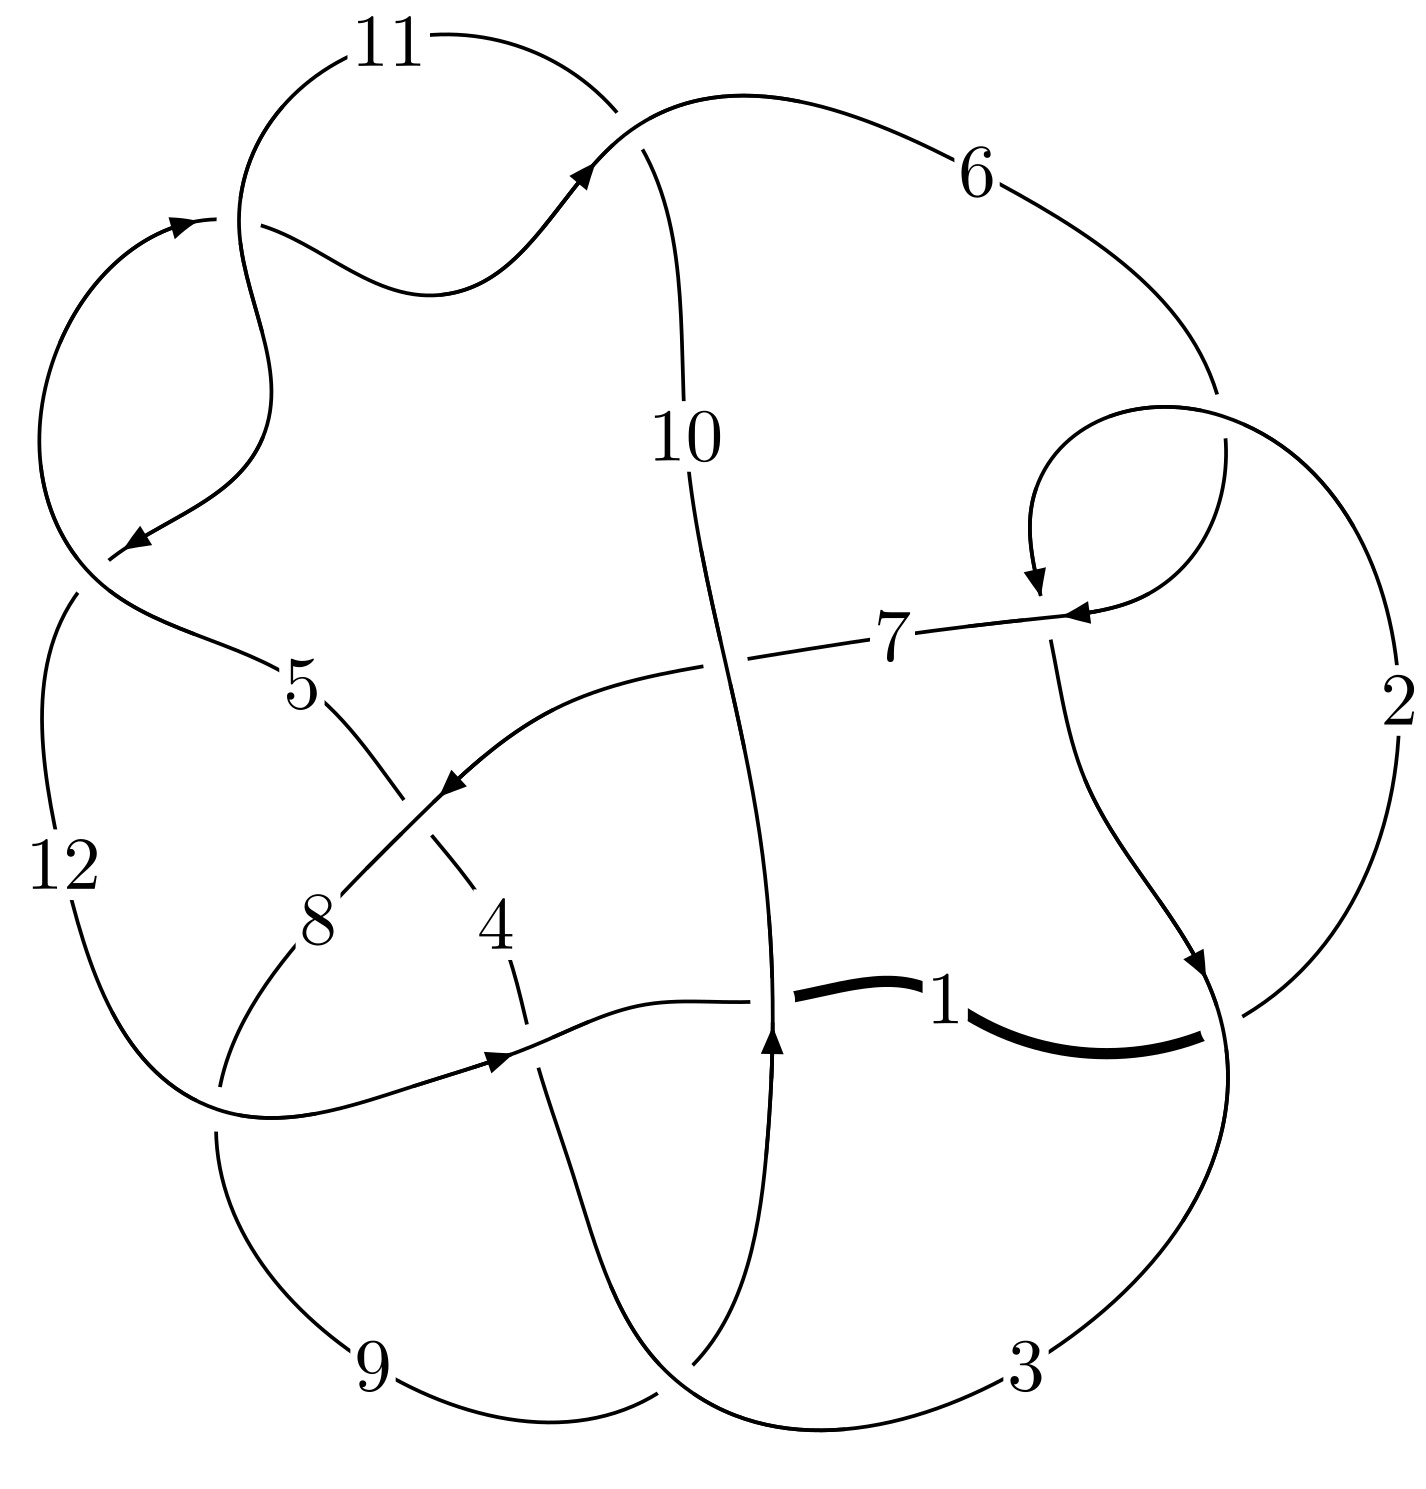
\includegraphics[width=112pt]{../../../GIT/diagram.site/Diagrams/png/2650_12n_0561.png}\\
\ \ \ A knot diagram\footnotemark}&
\allowdisplaybreaks
\textbf{Linearized knot diagam} \\
\cline{2-2}
 &
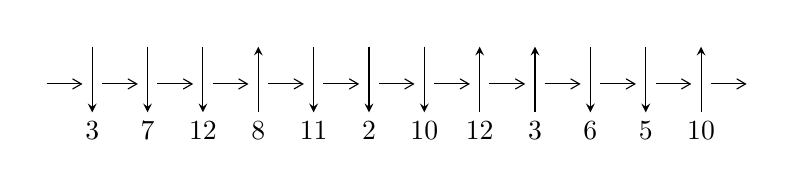
\begin{tikzpicture}[x=20pt, y=17pt]
	% nodes
	\node (C0) at (0, 0) {};
	\node (C1) at (1, 0) {};
	\node (C1U) at (1, +1) {};
	\node (C1D) at (1, -1) {3};

	\node (C2) at (2, 0) {};
	\node (C2U) at (2, +1) {};
	\node (C2D) at (2, -1) {7};

	\node (C3) at (3, 0) {};
	\node (C3U) at (3, +1) {};
	\node (C3D) at (3, -1) {12};

	\node (C4) at (4, 0) {};
	\node (C4U) at (4, +1) {};
	\node (C4D) at (4, -1) {8};

	\node (C5) at (5, 0) {};
	\node (C5U) at (5, +1) {};
	\node (C5D) at (5, -1) {11};

	\node (C6) at (6, 0) {};
	\node (C6U) at (6, +1) {};
	\node (C6D) at (6, -1) {2};

	\node (C7) at (7, 0) {};
	\node (C7U) at (7, +1) {};
	\node (C7D) at (7, -1) {10};

	\node (C8) at (8, 0) {};
	\node (C8U) at (8, +1) {};
	\node (C8D) at (8, -1) {12};

	\node (C9) at (9, 0) {};
	\node (C9U) at (9, +1) {};
	\node (C9D) at (9, -1) {3};

	\node (C10) at (10, 0) {};
	\node (C10U) at (10, +1) {};
	\node (C10D) at (10, -1) {6};

	\node (C11) at (11, 0) {};
	\node (C11U) at (11, +1) {};
	\node (C11D) at (11, -1) {5};

	\node (C12) at (12, 0) {};
	\node (C12U) at (12, +1) {};
	\node (C12D) at (12, -1) {10};
	\node (C13) at (13, 0) {};

	% arrows
	\draw[->,>={angle 60}]
	(C0) edge (C1) (C1) edge (C2) (C2) edge (C3) (C3) edge (C4) (C4) edge (C5) (C5) edge (C6) (C6) edge (C7) (C7) edge (C8) (C8) edge (C9) (C9) edge (C10) (C10) edge (C11) (C11) edge (C12) (C12) edge (C13) ;	\draw[->,>=stealth]
	(C1U) edge (C1D) (C2U) edge (C2D) (C3U) edge (C3D) (C4D) edge (C4U) (C5U) edge (C5D) (C6U) edge (C6D) (C7U) edge (C7D) (C8D) edge (C8U) (C9D) edge (C9U) (C10U) edge (C10D) (C11U) edge (C11D) (C12D) edge (C12U) ;
	\end{tikzpicture} \\
\hhline{~~} \\& 
\textbf{Solving Sequence} \\ \cline{2-2} 
 &
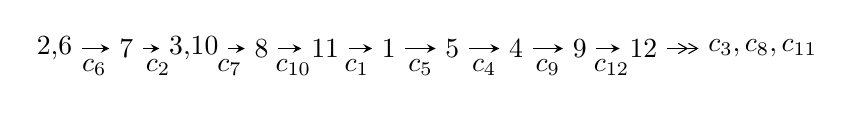
\begin{tikzpicture}[x=23pt, y=7pt]
	% node
	\node (A0) at (-1/8, 0) {2,6};
	\node (A1) at (1, 0) {7};
	\node (A2) at (33/16, 0) {3,10};
	\node (A3) at (25/8, 0) {8};
	\node (A4) at (33/8, 0) {11};
	\node (A5) at (41/8, 0) {1};
	\node (A6) at (49/8, 0) {5};
	\node (A7) at (57/8, 0) {4};
	\node (A8) at (65/8, 0) {9};
	\node (A9) at (73/8, 0) {12};
	\node (C1) at (1/2, -1) {$c_{6}$};
	\node (C2) at (3/2, -1) {$c_{2}$};
	\node (C3) at (21/8, -1) {$c_{7}$};
	\node (C4) at (29/8, -1) {$c_{10}$};
	\node (C5) at (37/8, -1) {$c_{1}$};
	\node (C6) at (45/8, -1) {$c_{5}$};
	\node (C7) at (53/8, -1) {$c_{4}$};
	\node (C8) at (61/8, -1) {$c_{9}$};
	\node (C9) at (69/8, -1) {$c_{12}$};
	\node (A10) at (11, 0) {$c_{3},c_{8},c_{11}$};

	% edge
	\draw[->,>=stealth]	
	(A0) edge (A1) (A1) edge (A2) (A2) edge (A3) (A3) edge (A4) (A4) edge (A5) (A5) edge (A6) (A6) edge (A7) (A7) edge (A8) (A8) edge (A9) ;
	\draw[->>,>={angle 60}]	
	(A9) edge (A10);
\end{tikzpicture} \\ 

\end{tabular} \\

\footnotetext{
The image of knot diagram is generated by the software ``\textbf{Draw programme}" developed by Andrew Bartholomew(\url{http://www.layer8.co.uk/maths/draw/index.htm\#Running-draw}), where we modified some parts for our purpose(\url{https://github.com/CATsTAILs/LinksPainter}).
}\phantom \\ \newline 
\centering \textbf{Ideals for irreducible components\footnotemark of $X_{\text{par}}$} 
 
\begin{align*}
I^u_{1}&=\langle 
19514643174787 u^{34}-4572969237385 u^{33}+\cdots+35208391096192 b-115134997157437,\\
\phantom{I^u_{1}}&\phantom{= \langle  }-44181034772241 u^{34}-93208096612611 u^{33}+\cdots+176041955480960 a-34686663928811,\\
\phantom{I^u_{1}}&\phantom{= \langle  }u^{35}+u^{34}+\cdots-4 u-5\rangle \\
I^u_{2}&=\langle 
- u^2 a- u^2+b+a,\;u^3 a-2 u^2 a+u^3+a^2- a u+2 a-1,\;u^4- u^2+1\rangle \\
\\
\end{align*}
\raggedright * 2 irreducible components of $\dim_{\mathbb{C}}=0$, with total 43 representations.\\
\footnotetext{All coefficients of polynomials are rational numbers. But the coefficients are sometimes approximated in decimal forms when there is not enough margin.}
\newpage
\renewcommand{\arraystretch}{1}
\centering \section*{I. $I^u_{1}= \langle 1.95\times10^{13} u^{34}-4.57\times10^{12} u^{33}+\cdots+3.52\times10^{13} b-1.15\times10^{14},\;-4.42\times10^{13} u^{34}-9.32\times10^{13} u^{33}+\cdots+1.76\times10^{14} a-3.47\times10^{13},\;u^{35}+u^{34}+\cdots-4 u-5 \rangle$}
\flushleft \textbf{(i) Arc colorings}\\
\begin{tabular}{m{7pt} m{180pt} m{7pt} m{180pt} }
\flushright $a_{2}=$&$\begin{pmatrix}0\\u\end{pmatrix}$ \\
\flushright $a_{6}=$&$\begin{pmatrix}1\\0\end{pmatrix}$ \\
\flushright $a_{7}=$&$\begin{pmatrix}1\\u^2\end{pmatrix}$ \\
\flushright $a_{3}=$&$\begin{pmatrix}- u\\- u^3+u\end{pmatrix}$ \\
\flushright $a_{10}=$&$\begin{pmatrix}0.250969 u^{34}+0.529465 u^{33}+\cdots+2.80218 u+0.197036\\-0.554261 u^{34}+0.129883 u^{33}+\cdots+0.868164 u+3.27010\end{pmatrix}$ \\
\flushright $a_{8}=$&$\begin{pmatrix}0.791772 u^{34}+0.423142 u^{33}+\cdots+3.34243 u-2.71039\\-0.523385 u^{34}+0.0869282 u^{33}+\cdots+0.937584 u+2.29735\end{pmatrix}$ \\
\flushright $a_{11}=$&$\begin{pmatrix}0.805230 u^{34}+0.399582 u^{33}+\cdots+1.93402 u-3.07306\\-0.554261 u^{34}+0.129883 u^{33}+\cdots+0.868164 u+3.27010\end{pmatrix}$ \\
\flushright $a_{1}=$&$\begin{pmatrix}u^3\\u^5- u^3+u\end{pmatrix}$ \\
\flushright $a_{5}=$&$\begin{pmatrix}-0.472936 u^{34}+0.0799123 u^{33}+\cdots+0.438637 u+2.87741\\-0.556115 u^{34}-0.173472 u^{33}+\cdots-2.34087 u+2.38011\end{pmatrix}$ \\
\flushright $a_{4}=$&$\begin{pmatrix}-0.816166 u^{34}+0.145199 u^{33}+\cdots+1.79451 u+3.42292\\-1.06658 u^{34}-0.102045 u^{33}+\cdots-3.07330 u+6.87995\end{pmatrix}$ \\
\flushright $a_{9}=$&$\begin{pmatrix}0.601350 u^{34}+0.306853 u^{33}+\cdots+2.54938 u-1.70567\\-0.455033 u^{34}+0.135445 u^{33}+\cdots+0.580899 u+2.30784\end{pmatrix}$ \\
\flushright $a_{12}=$&$\begin{pmatrix}-0.528222 u^{34}+0.0504600 u^{33}+\cdots-1.61488 u+4.49023\\0.662513 u^{34}+0.0170577 u^{33}+\cdots+1.34187 u-2.86220\end{pmatrix}$\\&\end{tabular}
\flushleft \textbf{(ii) Obstruction class $= -1$}\\~\\
\flushleft \textbf{(iii) Cusp Shapes $= -\frac{3308824036235}{17604195548096} u^{34}+\frac{2338411391075}{17604195548096} u^{33}+\cdots+\frac{68902332437973}{8802097774048} u-\frac{143545741438237}{17604195548096}$}\\~\\
\newpage\renewcommand{\arraystretch}{1}
\flushleft \textbf{(iv) u-Polynomials at the component}\newline \\
\begin{tabular}{m{50pt}|m{274pt}}
Crossings & \hspace{64pt}u-Polynomials at each crossing \\
\hline $$\begin{aligned}c_{1}\end{aligned}$$&$\begin{aligned}
&u^{35}+21 u^{34}+\cdots-74 u+25
\end{aligned}$\\
\hline $$\begin{aligned}c_{2},c_{6}\end{aligned}$$&$\begin{aligned}
&u^{35}- u^{34}+\cdots-4 u+5
\end{aligned}$\\
\hline $$\begin{aligned}c_{3}\end{aligned}$$&$\begin{aligned}
&u^{35}-5 u^{34}+\cdots+296 u+28
\end{aligned}$\\
\hline $$\begin{aligned}c_{4},c_{9}\end{aligned}$$&$\begin{aligned}
&u^{35}- u^{34}+\cdots-16 u+4
\end{aligned}$\\
\hline $$\begin{aligned}c_{5},c_{10},c_{11}\end{aligned}$$&$\begin{aligned}
&u^{35}+u^{34}+\cdots-6 u+1
\end{aligned}$\\
\hline $$\begin{aligned}c_{7}\end{aligned}$$&$\begin{aligned}
&u^{35}-3 u^{34}+\cdots+6720 u-1472
\end{aligned}$\\
\hline $$\begin{aligned}c_{8}\end{aligned}$$&$\begin{aligned}
&u^{35}-3 u^{34}+\cdots+6 u+5
\end{aligned}$\\
\hline $$\begin{aligned}c_{12}\end{aligned}$$&$\begin{aligned}
&u^{35}+3 u^{34}+\cdots+12 u+1
\end{aligned}$\\
\hline
\end{tabular}\\~\\
\newpage\renewcommand{\arraystretch}{1}
\flushleft \textbf{(v) Riley Polynomials at the component}\newline \\
\begin{tabular}{m{50pt}|m{274pt}}
Crossings & \hspace{64pt}Riley Polynomials at each crossing \\
\hline $$\begin{aligned}c_{1}\end{aligned}$$&$\begin{aligned}
&y^{35}-9 y^{34}+\cdots+39626 y-625
\end{aligned}$\\
\hline $$\begin{aligned}c_{2},c_{6}\end{aligned}$$&$\begin{aligned}
&y^{35}-21 y^{34}+\cdots-74 y-25
\end{aligned}$\\
\hline $$\begin{aligned}c_{3}\end{aligned}$$&$\begin{aligned}
&y^{35}-57 y^{34}+\cdots-32784 y-784
\end{aligned}$\\
\hline $$\begin{aligned}c_{4},c_{9}\end{aligned}$$&$\begin{aligned}
&y^{35}+43 y^{34}+\cdots+184 y-16
\end{aligned}$\\
\hline $$\begin{aligned}c_{5},c_{10},c_{11}\end{aligned}$$&$\begin{aligned}
&y^{35}+39 y^{34}+\cdots+34 y-1
\end{aligned}$\\
\hline $$\begin{aligned}c_{7}\end{aligned}$$&$\begin{aligned}
&y^{35}-31 y^{34}+\cdots+22678016 y-2166784
\end{aligned}$\\
\hline $$\begin{aligned}c_{8}\end{aligned}$$&$\begin{aligned}
&y^{35}+39 y^{34}+\cdots+126 y-25
\end{aligned}$\\
\hline $$\begin{aligned}c_{12}\end{aligned}$$&$\begin{aligned}
&y^{35}+51 y^{34}+\cdots+154 y-1
\end{aligned}$\\
\hline
\end{tabular}\\~\\
\newpage\flushleft \textbf{(vi) Complex Volumes and Cusp Shapes}
$$\begin{array}{c|c|c}  
\text{Solutions to }I^u_{1}& \I (\text{vol} + \sqrt{-1}CS) & \text{Cusp shape}\\
 \hline 
\begin{aligned}
u &= -0.203911 + 0.973360 I \\
a &= -0.519106 + 0.963683 I \\
b &= -0.26045 - 1.53546 I\end{aligned}
 & -1.43478 - 6.20512 I & -1.86669 + 2.78198 I \\ \hline\begin{aligned}
u &= -0.203911 - 0.973360 I \\
a &= -0.519106 - 0.963683 I \\
b &= -0.26045 + 1.53546 I\end{aligned}
 & -1.43478 + 6.20512 I & -1.86669 - 2.78198 I \\ \hline\begin{aligned}
u &= \phantom{-}0.066320 + 0.984954 I \\
a &= -0.448541 - 0.317717 I \\
b &= -0.750046 + 0.533829 I\end{aligned}
 & -8.19601 + 2.49744 I & -5.06408 - 2.60195 I \\ \hline\begin{aligned}
u &= \phantom{-}0.066320 - 0.984954 I \\
a &= -0.448541 + 0.317717 I \\
b &= -0.750046 - 0.533829 I\end{aligned}
 & -8.19601 - 2.49744 I & -5.06408 + 2.60195 I \\ \hline\begin{aligned}
u &= \phantom{-}0.801249 + 0.559810 I \\
a &= \phantom{-}1.36028 - 1.03030 I \\
b &= \phantom{-}0.01451 + 1.59501 I\end{aligned}
 & \phantom{-}8.83899 - 2.24678 I & \phantom{-}4.64462 + 3.81835 I \\ \hline\begin{aligned}
u &= \phantom{-}0.801249 - 0.559810 I \\
a &= \phantom{-}1.36028 + 1.03030 I \\
b &= \phantom{-}0.01451 - 1.59501 I\end{aligned}
 & \phantom{-}8.83899 + 2.24678 I & \phantom{-}4.64462 - 3.81835 I \\ \hline\begin{aligned}
u &= \phantom{-}1.014440 + 0.137733 I \\
a &= -1.44237 + 0.41096 I \\
b &= -0.391237 + 0.679863 I\end{aligned}
 & -2.29834 - 0.76813 I & -7.21756 - 0.78239 I \\ \hline\begin{aligned}
u &= \phantom{-}1.014440 - 0.137733 I \\
a &= -1.44237 - 0.41096 I \\
b &= -0.391237 - 0.679863 I\end{aligned}
 & -2.29834 + 0.76813 I & -7.21756 + 0.78239 I \\ \hline\begin{aligned}
u &= \phantom{-}0.910408 + 0.541398 I \\
a &= -0.378721 + 0.991836 I \\
b &= -0.212665 - 0.039123 I\end{aligned}
 & -1.75949 - 2.05479 I & -11.09061 + 3.13209 I \\ \hline\begin{aligned}
u &= \phantom{-}0.910408 - 0.541398 I \\
a &= -0.378721 - 0.991836 I \\
b &= -0.212665 + 0.039123 I\end{aligned}
 & -1.75949 + 2.05479 I & -11.09061 - 3.13209 I\\
 \hline 
 \end{array}$$\newpage$$\begin{array}{c|c|c}  
\text{Solutions to }I^u_{1}& \I (\text{vol} + \sqrt{-1}CS) & \text{Cusp shape}\\
 \hline 
\begin{aligned}
u &= -0.922478 + 0.127300 I \\
a &= -1.96495 + 0.18361 I \\
b &= -0.05491 + 1.64507 I\end{aligned}
 & \phantom{-}5.90539 + 0.64255 I & -5.75392 + 0.64646 I \\ \hline\begin{aligned}
u &= -0.922478 - 0.127300 I \\
a &= -1.96495 - 0.18361 I \\
b &= -0.05491 - 1.64507 I\end{aligned}
 & \phantom{-}5.90539 - 0.64255 I & -5.75392 - 0.64646 I \\ \hline\begin{aligned}
u &= -0.812370 + 0.424392 I \\
a &= \phantom{-}0.773162 + 0.362489 I \\
b &= \phantom{-}0.109550 - 0.685718 I\end{aligned}
 & \phantom{-}1.05382 + 1.86722 I & \phantom{-}3.18128 - 4.59075 I \\ \hline\begin{aligned}
u &= -0.812370 - 0.424392 I \\
a &= \phantom{-}0.773162 - 0.362489 I \\
b &= \phantom{-}0.109550 + 0.685718 I\end{aligned}
 & \phantom{-}1.05382 - 1.86722 I & \phantom{-}3.18128 + 4.59075 I \\ \hline\begin{aligned}
u &= \phantom{-}0.912261\phantom{ +0.000000I} \\
a &= \phantom{-}1.05610\phantom{ +0.000000I} \\
b &= \phantom{-}0.463900\phantom{ +0.000000I}\end{aligned}
 & -1.34236\phantom{ +0.000000I} & -8.12570\phantom{ +0.000000I} \\ \hline\begin{aligned}
u &= -0.842169 + 0.777146 I \\
a &= -0.89892 - 1.28817 I \\
b &= -0.050273 + 1.397230 I\end{aligned}
 & \phantom{-}3.07114 + 2.89052 I & -2.21100 - 2.95071 I \\ \hline\begin{aligned}
u &= -0.842169 - 0.777146 I \\
a &= -0.89892 + 1.28817 I \\
b &= -0.050273 - 1.397230 I\end{aligned}
 & \phantom{-}3.07114 - 2.89052 I & -2.21100 + 2.95071 I \\ \hline\begin{aligned}
u &= -1.137850 + 0.335834 I \\
a &= -1.53286 + 0.05803 I \\
b &= -0.587577 + 0.359881 I\end{aligned}
 & -3.27817 + 4.26600 I & -8.05552 - 6.74990 I \\ \hline\begin{aligned}
u &= -1.137850 - 0.335834 I \\
a &= -1.53286 - 0.05803 I \\
b &= -0.587577 - 0.359881 I\end{aligned}
 & -3.27817 - 4.26600 I & -8.05552 + 6.74990 I \\ \hline\begin{aligned}
u &= -1.152990 + 0.388555 I \\
a &= \phantom{-}0.878906 - 1.034180 I \\
b &= \phantom{-}0.002872 - 1.337860 I\end{aligned}
 & \phantom{-}2.24498 + 1.33286 I & -3.24945 - 0.69819 I\\
 \hline 
 \end{array}$$\newpage$$\begin{array}{c|c|c}  
\text{Solutions to }I^u_{1}& \I (\text{vol} + \sqrt{-1}CS) & \text{Cusp shape}\\
 \hline 
\begin{aligned}
u &= -1.152990 - 0.388555 I \\
a &= \phantom{-}0.878906 + 1.034180 I \\
b &= \phantom{-}0.002872 + 1.337860 I\end{aligned}
 & \phantom{-}2.24498 - 1.33286 I & -3.24945 + 0.69819 I \\ \hline\begin{aligned}
u &= \phantom{-}0.098226 + 0.753815 I \\
a &= \phantom{-}0.468379 + 0.420561 I \\
b &= \phantom{-}0.09057 - 1.46639 I\end{aligned}
 & \phantom{-}5.88674 + 2.52249 I & \phantom{-}1.23506 - 2.87985 I \\ \hline\begin{aligned}
u &= \phantom{-}0.098226 - 0.753815 I \\
a &= \phantom{-}0.468379 - 0.420561 I \\
b &= \phantom{-}0.09057 + 1.46639 I\end{aligned}
 & \phantom{-}5.88674 - 2.52249 I & \phantom{-}1.23506 + 2.87985 I \\ \hline\begin{aligned}
u &= \phantom{-}1.194500 + 0.470305 I \\
a &= -1.80401 - 0.60694 I \\
b &= -0.19201 - 1.46324 I\end{aligned}
 & \phantom{-}2.66330 - 7.05772 I & -2.51905 + 5.88692 I \\ \hline\begin{aligned}
u &= \phantom{-}1.194500 - 0.470305 I \\
a &= -1.80401 + 0.60694 I \\
b &= -0.19201 + 1.46324 I\end{aligned}
 & \phantom{-}2.66330 + 7.05772 I & -2.51905 - 5.88692 I \\ \hline\begin{aligned}
u &= \phantom{-}1.330550 + 0.340353 I \\
a &= \phantom{-}0.175592 - 0.683458 I \\
b &= \phantom{-}0.33732 - 1.47223 I\end{aligned}
 & -6.45071 + 1.73894 I & -5.86337 - 0.49500 I \\ \hline\begin{aligned}
u &= \phantom{-}1.330550 - 0.340353 I \\
a &= \phantom{-}0.175592 + 0.683458 I \\
b &= \phantom{-}0.33732 + 1.47223 I\end{aligned}
 & -6.45071 - 1.73894 I & -5.86337 + 0.49500 I \\ \hline\begin{aligned}
u &= -1.252450 + 0.585255 I \\
a &= \phantom{-}1.89880 + 0.08113 I \\
b &= \phantom{-}0.27080 - 1.59119 I\end{aligned}
 & -4.64525 + 11.83980 I & -4.29756 - 5.89282 I \\ \hline\begin{aligned}
u &= -1.252450 - 0.585255 I \\
a &= \phantom{-}1.89880 - 0.08113 I \\
b &= \phantom{-}0.27080 + 1.59119 I\end{aligned}
 & -4.64525 - 11.83980 I & -4.29756 + 5.89282 I \\ \hline\begin{aligned}
u &= -1.326130 + 0.448294 I \\
a &= \phantom{-}0.903307 + 0.583518 I \\
b &= \phantom{-}0.842224 + 0.446428 I\end{aligned}
 & -12.58030 + 2.55008 I & -8.43526 - 0.60252 I\\
 \hline 
 \end{array}$$\newpage$$\begin{array}{c|c|c}  
\text{Solutions to }I^u_{1}& \I (\text{vol} + \sqrt{-1}CS) & \text{Cusp shape}\\
 \hline 
\begin{aligned}
u &= -1.326130 - 0.448294 I \\
a &= \phantom{-}0.903307 - 0.583518 I \\
b &= \phantom{-}0.842224 - 0.446428 I\end{aligned}
 & -12.58030 - 2.55008 I & -8.43526 + 0.60252 I \\ \hline\begin{aligned}
u &= \phantom{-}1.297550 + 0.525631 I \\
a &= \phantom{-}1.45281 - 0.36988 I \\
b &= \phantom{-}0.780540 + 0.640043 I\end{aligned}
 & -11.9977 - 7.9047 I & -7.36295 + 5.50788 I \\ \hline\begin{aligned}
u &= \phantom{-}1.297550 - 0.525631 I \\
a &= \phantom{-}1.45281 + 0.36988 I \\
b &= \phantom{-}0.780540 - 0.640043 I\end{aligned}
 & -11.9977 + 7.9047 I & -7.36295 - 5.50788 I \\ \hline\begin{aligned}
u &= -0.019019 + 0.438455 I \\
a &= \phantom{-}0.850181 + 0.183537 I \\
b &= \phantom{-}0.318829 + 0.391878 I\end{aligned}
 & -0.204022 - 1.109310 I & -3.01108 + 6.25704 I \\ \hline\begin{aligned}
u &= -0.019019 - 0.438455 I \\
a &= \phantom{-}0.850181 - 0.183537 I \\
b &= \phantom{-}0.318829 - 0.391878 I\end{aligned}
 & -0.204022 + 1.109310 I & -3.01108 - 6.25704 I\\
 \hline 
 \end{array}$$\newpage\newpage\renewcommand{\arraystretch}{1}
\centering \section*{II. $I^u_{2}= \langle - u^2 a- u^2+b+a,\;u^3 a-2 u^2 a+u^3+a^2- a u+2 a-1,\;u^4- u^2+1 \rangle$}
\flushleft \textbf{(i) Arc colorings}\\
\begin{tabular}{m{7pt} m{180pt} m{7pt} m{180pt} }
\flushright $a_{2}=$&$\begin{pmatrix}0\\u\end{pmatrix}$ \\
\flushright $a_{6}=$&$\begin{pmatrix}1\\0\end{pmatrix}$ \\
\flushright $a_{7}=$&$\begin{pmatrix}1\\u^2\end{pmatrix}$ \\
\flushright $a_{3}=$&$\begin{pmatrix}- u\\- u^3+u\end{pmatrix}$ \\
\flushright $a_{10}=$&$\begin{pmatrix}a\\u^2 a+u^2- a\end{pmatrix}$ \\
\flushright $a_{8}=$&$\begin{pmatrix}u^3 a- u^2 a+u^3- a u+2 a\\- u^3 a+u^2 a+u^2- a- u\end{pmatrix}$ \\
\flushright $a_{11}=$&$\begin{pmatrix}- u^2 a- u^2+2 a\\u^2 a+u^2- a\end{pmatrix}$ \\
\flushright $a_{1}=$&$\begin{pmatrix}u^3\\0\end{pmatrix}$ \\
\flushright $a_{5}=$&$\begin{pmatrix}- u^3 a+u^2 a+u^3- a u- u^2-2 u+1\\- u^3+a u+u+1\end{pmatrix}$ \\
\flushright $a_{4}=$&$\begin{pmatrix}-2 u^3 a+2 u^2 a+u^3-2 a u- u^2-2 u+2\\-2 u^3+2 a u+u^2- a+2 u\end{pmatrix}$ \\
\flushright $a_{9}=$&$\begin{pmatrix}- u^2+a+1\\u^2 a+2 u^2- a\end{pmatrix}$ \\
\flushright $a_{12}=$&$\begin{pmatrix}- u^3 a+u^3+a u+u^2- a- u-1\\- u^2 a- u^3- u^2+a\end{pmatrix}$\\&\end{tabular}
\flushleft \textbf{(ii) Obstruction class $= 1$}\\~\\
\flushleft \textbf{(iii) Cusp Shapes $= 4 u^2-4$}\\~\\
\newpage\renewcommand{\arraystretch}{1}
\flushleft \textbf{(iv) u-Polynomials at the component}\newline \\
\begin{tabular}{m{50pt}|m{274pt}}
Crossings & \hspace{64pt}u-Polynomials at each crossing \\
\hline $$\begin{aligned}c_{1}\end{aligned}$$&$\begin{aligned}
&(u^2- u+1)^4
\end{aligned}$\\
\hline $$\begin{aligned}c_{2},c_{6},c_{8}\end{aligned}$$&$\begin{aligned}
&(u^4- u^2+1)^2
\end{aligned}$\\
\hline $$\begin{aligned}c_{3}\end{aligned}$$&$\begin{aligned}
&u^8+4 u^7+16 u^6+34 u^5+57 u^4+62 u^3+46 u^2+20 u+4
\end{aligned}$\\
\hline $$\begin{aligned}c_{4},c_{9}\end{aligned}$$&$\begin{aligned}
&(u^2+1)^4
\end{aligned}$\\
\hline $$\begin{aligned}c_{5},c_{10},c_{11}\end{aligned}$$&$\begin{aligned}
&(u^4+3 u^2+1)^2
\end{aligned}$\\
\hline $$\begin{aligned}c_{7}\end{aligned}$$&$\begin{aligned}
&u^8-8 u^7+25 u^6-38 u^5+33 u^4-28 u^3+28 u^2-16 u+4
\end{aligned}$\\
\hline $$\begin{aligned}c_{12}\end{aligned}$$&$\begin{aligned}
&(u^2+u-1)^4
\end{aligned}$\\
\hline
\end{tabular}\\~\\
\newpage\renewcommand{\arraystretch}{1}
\flushleft \textbf{(v) Riley Polynomials at the component}\newline \\
\begin{tabular}{m{50pt}|m{274pt}}
Crossings & \hspace{64pt}Riley Polynomials at each crossing \\
\hline $$\begin{aligned}c_{1}\end{aligned}$$&$\begin{aligned}
&(y^2+y+1)^4
\end{aligned}$\\
\hline $$\begin{aligned}c_{2},c_{6},c_{8}\end{aligned}$$&$\begin{aligned}
&(y^2- y+1)^4
\end{aligned}$\\
\hline $$\begin{aligned}c_{3}\end{aligned}$$&$\begin{aligned}
&y^8+16 y^7+98 y^6+264 y^5+353 y^4+168 y^3+92 y^2-32 y+16
\end{aligned}$\\
\hline $$\begin{aligned}c_{4},c_{9}\end{aligned}$$&$\begin{aligned}
&(y+1)^8
\end{aligned}$\\
\hline $$\begin{aligned}c_{5},c_{10},c_{11}\end{aligned}$$&$\begin{aligned}
&(y^2+3 y+1)^4
\end{aligned}$\\
\hline $$\begin{aligned}c_{7}\end{aligned}$$&$\begin{aligned}
&y^8-14 y^7+83 y^6-186 y^5+113 y^4+48 y^3+152 y^2-32 y+16
\end{aligned}$\\
\hline $$\begin{aligned}c_{12}\end{aligned}$$&$\begin{aligned}
&(y^2-3 y+1)^4
\end{aligned}$\\
\hline
\end{tabular}\\~\\
\newpage\flushleft \textbf{(vi) Complex Volumes and Cusp Shapes}
$$\begin{array}{c|c|c}  
\text{Solutions to }I^u_{2}& \I (\text{vol} + \sqrt{-1}CS) & \text{Cusp shape}\\
 \hline 
\begin{aligned}
u &= \phantom{-}0.866025 + 0.500000 I \\
a &= \phantom{-}0.901259 + 0.057008 I \\
b &= \phantom{-0.000000 -}1.61803 I\end{aligned}
 & \phantom{-}7.23771 - 2.02988 I & -2.00000 + 3.46410 I \\ \hline\begin{aligned}
u &= \phantom{-}0.866025 + 0.500000 I \\
a &= -1.03523 + 1.17504 I \\
b &= \phantom{-0.000000 } -0.618034 I\end{aligned}
 & -0.65797 - 2.02988 I & -2.00000 + 3.46410 I \\ \hline\begin{aligned}
u &= \phantom{-}0.866025 - 0.500000 I \\
a &= \phantom{-}0.901259 - 0.057008 I \\
b &= \phantom{-0.000000 } -1.61803 I\end{aligned}
 & \phantom{-}7.23771 + 2.02988 I & -2.00000 - 3.46410 I \\ \hline\begin{aligned}
u &= \phantom{-}0.866025 - 0.500000 I \\
a &= -1.03523 - 1.17504 I \\
b &= \phantom{-0.000000 -}0.618034 I\end{aligned}
 & -0.65797 + 2.02988 I & -2.00000 - 3.46410 I \\ \hline\begin{aligned}
u &= -0.866025 + 0.500000 I \\
a &= \phantom{-}0.035233 - 0.557008 I \\
b &= \phantom{-0.000000 } -0.618034 I\end{aligned}
 & -0.65797 + 2.02988 I & -2.00000 - 3.46410 I \\ \hline\begin{aligned}
u &= -0.866025 + 0.500000 I \\
a &= -1.90126 - 1.67504 I \\
b &= \phantom{-0.000000 -}1.61803 I\end{aligned}
 & \phantom{-}7.23771 + 2.02988 I & -2.00000 - 3.46410 I \\ \hline\begin{aligned}
u &= -0.866025 - 0.500000 I \\
a &= \phantom{-}0.035233 + 0.557008 I \\
b &= \phantom{-0.000000 -}0.618034 I\end{aligned}
 & -0.65797 - 2.02988 I & -2.00000 + 3.46410 I \\ \hline\begin{aligned}
u &= -0.866025 - 0.500000 I \\
a &= -1.90126 + 1.67504 I \\
b &= \phantom{-0.000000 } -1.61803 I\end{aligned}
 & \phantom{-}7.23771 - 2.02988 I & -2.00000 + 3.46410 I\\
 \hline 
 \end{array}$$\newpage
\newpage\renewcommand{\arraystretch}{1}
\centering \section*{ III. u-Polynomials}
\begin{tabular}{m{50pt}|m{274pt}}
Crossings & \hspace{64pt}u-Polynomials at each crossing \\
\hline $$\begin{aligned}c_{1}\end{aligned}$$&$\begin{aligned}
&((u^2- u+1)^4)(u^{35}+21 u^{34}+\cdots-74 u+25)
\end{aligned}$\\
\hline $$\begin{aligned}c_{2},c_{6}\end{aligned}$$&$\begin{aligned}
&((u^4- u^2+1)^2)(u^{35}- u^{34}+\cdots-4 u+5)
\end{aligned}$\\
\hline $$\begin{aligned}c_{3}\end{aligned}$$&$\begin{aligned}
&(u^8+4 u^7+16 u^6+34 u^5+57 u^4+62 u^3+46 u^2+20 u+4)\\
&\cdot(u^{35}-5 u^{34}+\cdots+296 u+28)
\end{aligned}$\\
\hline $$\begin{aligned}c_{4},c_{9}\end{aligned}$$&$\begin{aligned}
&((u^2+1)^4)(u^{35}- u^{34}+\cdots-16 u+4)
\end{aligned}$\\
\hline $$\begin{aligned}c_{5},c_{10},c_{11}\end{aligned}$$&$\begin{aligned}
&((u^4+3 u^2+1)^2)(u^{35}+u^{34}+\cdots-6 u+1)
\end{aligned}$\\
\hline $$\begin{aligned}c_{7}\end{aligned}$$&$\begin{aligned}
&(u^8-8 u^7+25 u^6-38 u^5+33 u^4-28 u^3+28 u^2-16 u+4)\\
&\cdot(u^{35}-3 u^{34}+\cdots+6720 u-1472)
\end{aligned}$\\
\hline $$\begin{aligned}c_{8}\end{aligned}$$&$\begin{aligned}
&((u^4- u^2+1)^2)(u^{35}-3 u^{34}+\cdots+6 u+5)
\end{aligned}$\\
\hline $$\begin{aligned}c_{12}\end{aligned}$$&$\begin{aligned}
&((u^2+u-1)^4)(u^{35}+3 u^{34}+\cdots+12 u+1)
\end{aligned}$\\
\hline
\end{tabular}\newpage\renewcommand{\arraystretch}{1}
\centering \section*{ IV. Riley Polynomials}
\begin{tabular}{m{50pt}|m{274pt}}
Crossings & \hspace{64pt}Riley Polynomials at each crossing \\
\hline $$\begin{aligned}c_{1}\end{aligned}$$&$\begin{aligned}
&((y^2+y+1)^4)(y^{35}-9 y^{34}+\cdots+39626 y-625)
\end{aligned}$\\
\hline $$\begin{aligned}c_{2},c_{6}\end{aligned}$$&$\begin{aligned}
&((y^2- y+1)^4)(y^{35}-21 y^{34}+\cdots-74 y-25)
\end{aligned}$\\
\hline $$\begin{aligned}c_{3}\end{aligned}$$&$\begin{aligned}
&(y^8+16 y^7+98 y^6+264 y^5+353 y^4+168 y^3+92 y^2-32 y+16)\\
&\cdot(y^{35}-57 y^{34}+\cdots-32784 y-784)
\end{aligned}$\\
\hline $$\begin{aligned}c_{4},c_{9}\end{aligned}$$&$\begin{aligned}
&((y+1)^8)(y^{35}+43 y^{34}+\cdots+184 y-16)
\end{aligned}$\\
\hline $$\begin{aligned}c_{5},c_{10},c_{11}\end{aligned}$$&$\begin{aligned}
&((y^2+3 y+1)^4)(y^{35}+39 y^{34}+\cdots+34 y-1)
\end{aligned}$\\
\hline $$\begin{aligned}c_{7}\end{aligned}$$&$\begin{aligned}
&(y^8-14 y^7+83 y^6-186 y^5+113 y^4+48 y^3+152 y^2-32 y+16)\\
&\cdot(y^{35}-31 y^{34}+\cdots+22678016 y-2166784)
\end{aligned}$\\
\hline $$\begin{aligned}c_{8}\end{aligned}$$&$\begin{aligned}
&((y^2- y+1)^4)(y^{35}+39 y^{34}+\cdots+126 y-25)
\end{aligned}$\\
\hline $$\begin{aligned}c_{12}\end{aligned}$$&$\begin{aligned}
&((y^2-3 y+1)^4)(y^{35}+51 y^{34}+\cdots+154 y-1)
\end{aligned}$\\
\hline
\end{tabular}
\vskip 2pc
\end{document}